\documentclass[authoryear,preprint,3p,review,10pt]{elsarticle}

%% Use the options 1p,twocolumn; 3p; 3p,twocolumn; 5p; or 5p,twocolumn
%% for a journal layout:
% \documentclass[final,1p,times,authoryear]{elsarticle}
%% \documentclass[final,1p,times,twocolumn,authoryear]{elsarticle}
% \documentclass[final,3p,times,authoryear]{elsarticle}
%% \documentclass[final,3p,times,twocolumn,authoryear]{elsarticle}
%% \documentclass[final,5p,times,authoryear]{elsarticle}
%% \documentclass[final,5p,times,twocolumn,authoryear]{elsarticle}

%% For including figures, graphicx.sty has been loaded in
%% elsarticle.cls. If you prefer to use the old commands
%% please give \usepackage{epsfig}


%% The amssymb package provides various useful mathematical symbols
\usepackage{amssymb}
%% The amsthm package provides extended theorem environments
\usepackage{amsthm}
\usepackage{amsmath}
\usepackage{amsfonts}
\usepackage{multirow}
\usepackage{bbm}
\usepackage{amsfonts}
\usepackage{footnote}
%\usepackage{multicol}
%\usepackage{booktabs}
%\usepackage[flushleft]{threeparttable}
%\usepackage[font=small,labelfont=bf]{caption}
%\usepackage{graphicx}
%\usepackage{epstopdf}
\usepackage{subcaption}
%\usepackage{epsfig}
%\usepackage{enumitem}
%\usepackage{slashbox}
%\usepackage[sectionbib]{natbib}
%\usepackage{natbib}

\usepackage{todonotes}
\usepackage{comment}
\setcounter{page}{1}
\newtheorem{theorem}{Theorem}
\newtheorem{lemma}[theorem]{Lemma}
\newtheorem{proposition}[theorem]{Proposition}
\newtheorem{corollary}[theorem]{Corollary}

\theoremstyle{definition}
\newtheorem{remark}[theorem]{Remark}
\newtheorem{definition}[theorem]{Definition}
\newtheorem{example}[theorem]{Example}

\newcommand{\KS}{{\rm KS}}
\newcommand{\R}{\mathbb{R}}
\newcommand{\N}{\mathbb{N}}

\newcommand{\correction}[2]{\textcolor{red}{#1}\textcolor{blue}{#2}}


%\newcommand{\ifr}{\textsc{ifr}}
%\newcommand{\ifra}{\textsc{ifra}}

\newcommand{\E}{\mathbb{E}}
\newcommand{\G}{\mathbb{G}}
\newcommand{\F}{\mathbb{F}}
\usepackage{amssymb}
%% The amsthm package provides extended theorem environments
\usepackage{amsthm}
\usepackage{amsmath}
\usepackage{amsfonts}
\usepackage{multirow}
\usepackage{relsize}

\usepackage{amsfonts}
\usepackage{footnote}
%\usepackage{multicol}
%\usepackage{booktabs}
%\usepackage[flushleft]{threeparttable}
%\usepackage[font=small,labelfont=bf]{caption}
%\usepackage{graphicx}
%\usepackage{epstopdf}
\usepackage{subcaption}
%\usepackage{epsfig}
%\usepackage{enumitem}
%\usepackage{slashbox}
%\usepackage[sectionbib]{natbib}
%\usepackage{natbib}

\usepackage{todonotes}
\usepackage{comment}
%% The lineno packages adds line numbers. Start line numbering with
%% \begin{linenumbers}, end it with \end{linenumbers}. Or switch it on
%% for the whole article with \linenumbers.
%% \usepackage{lineno}








\begin{document}
	\subsection*{Generalized Order Statistics}
	
	Let \(F\) be a continuous cumulative distribution function with corresponding quantile function \(F^{-1}\), and let \((\gamma_i)_{i\geq 1}\) be a sequence of positive parameters. Let \(U_1,U_2,\ldots\) be independent random variables, each uniformly distributed on \((0,1)\).
	
	For each \(r\geq 1\), define
	\[
	U_{r,\tilde{\gamma}_r}
	:=1-\prod_{i=1}^{r}U_i^{1/\gamma_i},
	\qquad
	\tilde{\gamma}_r:=(\gamma_1,\ldots,\gamma_r).
	\]
	The sequence \(\bigl(U_{r,\tilde{\gamma}_r}\bigr)_{r\geq 1}\) is referred to as a sequence of \textit{uniform generalized order statistics} (U-GOS) associated with the parameter sequence \((\gamma_i)_{i\geq 1}\).
	
	The corresponding sequence of \textit{generalized order statistics} associated with \(F\) is defined by applying the quantile function \(F^{-1}\) to the uniform GOS. Specifically, for \(r\geq 1\), let
	
	\begin{equation}\label{GOS}
		X_{r,\tilde{\gamma}_r}
		:=F^{-1}\!\left(U_{r,\tilde{\gamma}_r}\right)
		=F^{-1}\!\left(
		1-\prod_{i=1}^{r}U_i^{1/\gamma_i}
		\right).
	\end{equation}
	
	Thus, \(X_{r,\tilde{\gamma}_r}\) has the distribution induced by \(F^{-1}\) acting on the corresponding uniform GOS.
	
	
	
	\subsection*{Basic Properties}
	
	\begin{itemize}
		\item The sequence $(X_{r,\tilde{\gamma}_r})_{r \ge 1}$ is almost surely increasing:
		\[
		X_{1,\tilde{\gamma}_1} \le X_{2,\tilde{\gamma}_2} \le \cdots
		\]
		since the product $\prod_{i=1}^{r} U_i^{1/\gamma_i}$ is decreasing in $r$.
		
		\item The distribution of $X_{r,\tilde{\gamma}_r}$ depends only on the first $r$ parameters $(\gamma_1,\dots,\gamma_r)$.
		
		\item The construction is invariant under permutations of $(\gamma_1,\dots,\gamma_r)$ at the marginal level.
	\end{itemize}
	
	\subsection*{Special Cases}
	
	\begin{itemize}
		\item \textbf{Ordinary order statistics:}  
		If $\gamma_r = n+1-r$, $r=1,\dots,n$, then
		\[
		X_{r,\tilde{\gamma}_r} \equiv X_{r:n},
		\]
		the $r$-th order statistic of an i.i.d. sample of size $n$.
		
		\item \textbf{$k$-th upper record values:}  
		If $\gamma_i = k$ for all $i \ge 1$, then $(X_{r,\tilde{\gamma}_r})$ corresponds to the sequence of $k$-th upper record values. In particular, $k=1$ yields classical record values.
		
		\item \textbf{Progressively censored order statistics:}  
		For a censoring scheme $R=(R_1,\dots,R_n)$, the model corresponds to generalized order statistics with parameters
		\[
		\gamma_r = \sum_{i=r}^{n} (R_i + 1), \quad r=1,\dots,n.
		\]
	\end{itemize}
	
	
	The classes \(\mathcal{F}_G^{cx}\) and \(\mathcal{F}_G^{cv}\) can be characterized in terms of the expectation of the generalized order statistic (GOS), \(\mathbb{E}[X_{r,\tilde{\gamma}_r}]\). To make this characterization explicit, let
	\[
	U_{r,\tilde{\gamma}_r}
	=1-\prod_{i=1}^{r}U_i^{1/\gamma_i},
	\]
	where \(U_1,\ldots,U_r\) are independent random variables uniformly distributed on \((0,1)\), and define
	\[
	\mu_{r,\tilde{\gamma}_r}
	:=\mathbb{E}[X_{r,\tilde{\gamma}_r}],
	\qquad
	\pi_{r,\tilde{\gamma}_r}^{G}
	:=G\!\left(
	\mathbb{E}\!\left[
	G^{-1}(U_{r,\tilde{\gamma}_r})
	\right]\right).
	\]
	Assume that the relevant expectations exist and that \(G^{-1}\circ F\) is convex. By Jensen's inequality,
	\[
	\begin{aligned}
		(G^{-1}\circ F)
		\bigl(\mu_{r,\tilde{\gamma}_r}\bigr)
		&\leq
		\mathbb{E}\!\left[
		(G^{-1}\circ F)(X_{r,\tilde{\gamma}_r})
		\right]\\
		&=
		\mathbb{E}\!\left[
		G^{-1}(U_{r,\tilde{\gamma}_r})
		\right].
	\end{aligned}
	\]
	Applying \(G\) to both sides and using the monotonicity of \(G\), we obtain
	\[
	F\bigl(\mu_{r,\tilde{\gamma}_r}\bigr)
	\leq
	G\!\left(
	\mathbb{E}\!\left[
	G^{-1}(U_{r,\tilde{\gamma}_r})
	\right]\right)
	=
	\pi_{r,\tilde{\gamma}_r}^{G}.
	\]
	Consequently, the resulting bound depends only on \(G\), \(r\), and the parameter vector \(\tilde{\gamma}_r\), rather than on the particular distribution \(F\). The analogous argument for concave \(G^{-1}\circ F\) yields the reverse inequality. These observations lead to the following characterization.
	
	\begin{proposition}\label{prop}
		Let
		\[
		\pi_{r,\tilde{\gamma}_r}^{G}
		:=
		G\!\left(
		\mathbb{E}\!\left[
		G^{-1}(U_{r,\tilde{\gamma}_r})
		\right]\right),
		\]
		and suppose that the expectations involved are well-defined. Then, for every admissible \(r\) and parameter vector \(\tilde{\gamma}_r\),
		\begin{enumerate}
			\item If \(F\in\mathcal{F}_G^{cx}\), then
			\[
			\mathbb{P}\!\left(
			X\leq\mu_{r,\tilde{\gamma}_r}
			\right)
			\leq
			\pi_{r,\tilde{\gamma}_r}^{G}.
			\]
			
			\item If \(F\in\mathcal{F}_G^{cv}\), then
			\[
			\mathbb{P}\!\left(
			X\leq\mu_{r,\tilde{\gamma}_r}
			\right)
			\geq
			\pi_{r,\tilde{\gamma}_r}^{G}.
			\]
		\end{enumerate}
	\end{proposition}
	
	
	
	
	
	
	\section{Estimating the Expected Generalized Order Statistics}
	
	
	
	Recall from \eqref{GOS} that the generalized order statistic
	\(X_{r,\tilde{\gamma}_r}\) is defined by
	\[
	X_{r,\tilde{\gamma}_r}
	=F^{-1}\!\left(U_{r,\tilde{\gamma}_r}\right),
	\]
	where \(U_{r,\tilde{\gamma}_r}\) denotes the corresponding uniform generalized order statistic. Accordingly, its distribution function can be expressed as
	\begin{equation}\label{eq:GOS_cdf}
		F_{X_{r,\tilde{\gamma}_r}}(x)
		=F_{U_{r,\tilde{\gamma}_r}}\!\left(F(x)\right),
		\qquad x\in\mathbb{R}.
	\end{equation}
	This representation allows us to derive the distribution of
	\(X_{r,\tilde{\gamma}_r}\) directly from the distribution of its
	uniform counterpart.
	
	The goal now is to estimate the expected generalized order statistic $\mu_{r,\tilde{\gamma}_r}
	:=\mathbb{E}\!\left[X_{r,\tilde{\gamma}_r}\right].$ To facilitate this estimation, we first obtain explicit expressions for the distribution function in \eqref{eq:GOS_cdf}. We consider two important cases, according to the structure of the parameter vector \(\tilde{\gamma}_r=(\gamma_1,\ldots,\gamma_r)\): \textbf{Distinct parameters:}
	The parameters \(\gamma_1,\ldots,\gamma_r\) are pairwise distinct and \textbf{Equal parameters:}
	All parameters coincide, so that
	\(\gamma_1=\cdots=\gamma_r=k\). The latter case corresponds to upper
	record values under the associated parameterization. The following two lemmas establish the explicit distribution functions
	for these cases. 
	
	
	\begin{lemma}\label{cdf_U}
		suppose that \(\gamma_1,\ldots,\gamma_r\) are pairwise distinct positive real numbers. Then:
		\begin{itemize}
			
			
			\item The distribution function of \(U_{r,\tilde{\gamma}_r}\) is given by
			\[
			F_{U_{r,\tilde{\gamma}_r}}(u)=
			\begin{cases}
				0, & u\le 0,\\[6pt]
				1-\displaystyle\sum_{i=1}^{r}
				\left(
				\prod_{\substack{j=1\\j\ne i}}^{r}
				\frac{\gamma_j}{\gamma_j-\gamma_i}
				\right)(1-u)^{\gamma_i},
				& 0<u<1,\\[12pt]
				1, & u\ge 1.
			\end{cases}
			\]
			
			
			\item The probability density function of \(U_{r,\tilde{\gamma}_r}\) is given by
			\[
			f_{U_{r,\tilde{\gamma}_r}}(u)=
			\begin{cases}
				\displaystyle
				\sum_{i=1}^{r}
				\gamma_i
				\left(
				\prod_{\substack{j=1\\j\ne i}}^{r}
				\frac{\gamma_j}{\gamma_j-\gamma_i}
				\right)
				(1-u)^{\gamma_i-1},
				& 0<u<1,\\[12pt]
				0, & \text{otherwise}.
			\end{cases}
			\]
			
		\end{itemize}
	\end{lemma}
	\begin{lemma}\label{CDF_record}
		\begin{itemize}
			\item The distribution function of the $k$-th uniform record value $U_{r,\tilde{\gamma}_r}=1-\prod_{j=1}^{r}U_j^{1/k}$ is given by: $F_{U_{r,\tilde{\gamma}_r}}(u)=F_{\operatorname{Gamma}(r,1)}(-k\ln(1-u)).$
			
			
			\item The density $f_{U_{r,\tilde{\gamma}_r}}$ is bounded if and only if $k\ge2\quad$ or $\quad (k=1,\ r=1).$
		\end{itemize}
	\end{lemma}
	
	```latex
	\subsection{A Plug-in Estimator of the Expected Generalized Order Statistic}
	
	Let \(X_1,\ldots,X_n\) be an i.i.d.\ sample from a distribution function
	\(F\), and let \(F_n\) denote the corresponding empirical distribution
	function,
	\[
	F_n(x)=\frac{1}{n}\sum_{i=1}^{n}\mathbf{1}\{X_i\leq x\},
	\qquad x\in\mathbb{R}.
	\]
	Throughout, we use \(F_n\) to denote the empirical distribution function
	associated with the observed sample, whereas \(\mathbb{F}_n\) may be used
	when emphasizing its random nature.
	
	Recall that the distribution function of the generalized order
	statistic \(X_{r,\tilde{\gamma}_r}\) is given by
	\[
	F_{X_{r,\tilde{\gamma}_r}}(x)
	=\left(F_{U_{r,\tilde{\gamma}_r}}\circ F\right)(x),
	\]
	where \(F_{U_{r,\tilde{\gamma}_r}}\) is the distribution function of
	the uniform generalized order statistic
	\[
	U_{r,\tilde{\gamma}_r}
	\overset{d}{=}
	1-\prod_{j=1}^{r}U_j^{1/\gamma_j},
	\]
	with \(U_1,\ldots,U_r\) independent and uniformly distributed on
	\((0,1)\), and
	\(\tilde{\gamma}_r=(\gamma_1,\ldots,\gamma_r)\).
	
	Replacing the unknown distribution function \(F\) with its empirical
	counterpart \(F_n\) yields the plug-in estimator of the distribution
	function of \(X_{r,\tilde{\gamma}_r}\):
	\[
	\widehat F_{X_{r,\tilde{\gamma}_r}}(x)
	:=
	F_{U_{r,\tilde{\gamma}_r}}\!\left(F_n(x)\right).
	\]
	Consequently, provided the expectation exists, the expected generalized
	order statistic can be written as
	\[
	\mu_{r,\tilde{\gamma}_r}(F)
	:=\mathbb{E}\!\left[X_{r,\tilde{\gamma}_r}\right]
	=\int_{\mathbb{R}}
	x\,dF_{X_{r,\tilde{\gamma}_r}}(x).
	\]
	This representation motivates the following plug-in estimator:
	\[
	\begin{aligned}
		\widehat{\mu}_{r,\tilde{\gamma}_r}
		&:=\mu_{r,\tilde{\gamma}_r}(F_n)\\
		&=\int_{\mathbb{R}}x\,
		dF_{U_{r,\tilde{\gamma}_r}}\!\left(F_n(x)\right).
	\end{aligned}
	\]
	
	To obtain an explicit expression, let
	\[
	X_{(1:n)}\leq X_{(2:n)}\leq\cdots\leq X_{(n:n)}
	\]
	denote the sample order statistics. Since the empirical distribution
	function increases in increments of \(1/n\), the composed distribution
	function \(F_{U_{r,\tilde{\gamma}_r}}\circ F_n\) assigns the weight
	\[
	w_{i,n}^{(r,\tilde{\gamma}_r)}
	:=
	F_{U_{r,\tilde{\gamma}_r}}\!\left(\frac{i}{n}\right)
	-
	F_{U_{r,\tilde{\gamma}_r}}\!\left(\frac{i-1}{n}\right)
	\]
	to the \(i\)-th sample order statistic. It follows that
	\begin{equation}\label{eq:gos_mean_estimator}
		\boxed{
			\widehat{\mu}_{r,\tilde{\gamma}_r}
			=
			\sum_{i=1}^{n}
			X_{(i:n)}
			\left[
			F_{U_{r,\tilde{\gamma}_r}}\!\left(\frac{i}{n}\right)
			-
			F_{U_{r,\tilde{\gamma}_r}}\!\left(\frac{i-1}{n}\right)
			\right].
		}
	\end{equation}
	Equivalently, the weights admit the probabilistic representation
	\[
	w_{i,n}^{(r,\tilde{\gamma}_r)}
	=
	\mathbb{P}\!\left(
	\frac{i-1}{n}<U_{r,\tilde{\gamma}_r}\leq\frac{i}{n}
	\right).
	\]
	Since these weights are nonnegative and sum to one, the estimator
	\(\widehat{\mu}_{r,\tilde{\gamma}_r}\) is a weighted average of the
	sample order statistics.
	
	In particular, \(\widehat{\mu}_{r,\tilde{\gamma}_r}\) is an
	\(L\)-estimator, that is, a linear combination of order statistics
	whose weights are determined by the distribution of the corresponding
	uniform generalized order statistic. This representation is especially
	useful in practice because the weights depend only on
	\(r\), \(\tilde{\gamma}_r\), and the sample size \(n\), and can
	therefore be computed without knowing the underlying distribution
	function \(F\).
	```
	
	
	
	\section{The Tests}
	Our testing procedure is motivated by the inequalities established in Proposition \ref{prop}. Given the distribution function \(G\), the order \(r\), and the parameter vector \(\tilde{\gamma}_r\), the theoretical bound \(\pi_{r,\tilde{\gamma}_r}^{G}\) can be computed directly. This suggests a natural strategy: estimate the left-hand side of the corresponding inequality from the data and compare it with this theoretical bound.
	
	Let \(X_1,\ldots,X_n\) be a random sample from the distribution \(F\). We first estimate the expected generalized order statistic
	\[
	\mu_{r,\tilde{\gamma}_r}
	=\mathbb{E}\!\left[X_{r,\tilde{\gamma}_r}\right]
	\]
	by an estimator \(\widehat{\mu}_{r,\tilde{\gamma}_r}\). Here, the sample size \(n\) and the GOS index \(r\) are not necessarily equal. We then estimate the probability \(F(\mu_{r,\tilde{\gamma}_r})\) using the empirical distribution function evaluated at the estimated threshold:
	\[
	\widehat F_n\!\left(
	\widehat{\mu}_{r,\tilde{\gamma}_r}
	\right)
	=
	\frac{1}{n}\sum_{i=1}^{n}
	\mathbf{1}\!\left\{
	X_i\leq\widehat{\mu}_{r,\tilde{\gamma}_r}
	\right\}.
	\]
	Finally, we compare this empirical estimate with the deterministic \(\pi_{r,\tilde{\gamma}_r}^{G}\). To be more concret, let the following hypotheses
	
	
	To simplify notation, define the vectors
	\[
	\hat{\mathbf{V}}_r = \left( F_n(\widehat \mu_{1,\tilde\gamma_1}), \dots, F_n(\widehat{\mu}_{r,\tilde{\gamma_r}}) \right), \quad \text{and} \quad \mathbf{v}_r^G = \left( \pi_{1,\tilde{\gamma_1}}^G, \dots, \pi_{r,\tilde{\gamma_r}}^G \right).
	\]
	Thus, the test statistic for \( \mathcal{H}_{1+}^G \) is given by
	\[
	T_{r,\tilde \gamma_r,p}^{G+}(F_n) = \left\| \left( \mathbf{v}_r^G - \hat{\mathbf{V}}_r \right)_+ \right\|_p = \left( \sum_{k=1}^r \left( \pi_{k,\tilde{\gamma_k}}^G - F_n(\hat{\mu}_{k,\tilde{\gamma_k}}) \right)_+^p \right)^{1/p}.
	\]
	
	Similarly, to test \( \mathcal{H}_{1-}^G \), we define
	\[
	T_{r\tilde{\gamma_r},p}^{G-}(F_n) = \left\| \left( \mathbf{v}_r^G - \hat{\mathbf{V}}_r \right)_- \right\|_p.
	\]
	\section{Simulations}
	
	\begin{figure}[ht]
		\centering
		% --- First row: Weibull ---
		\begin{subfigure}[b]{\textwidth}
			\centering
			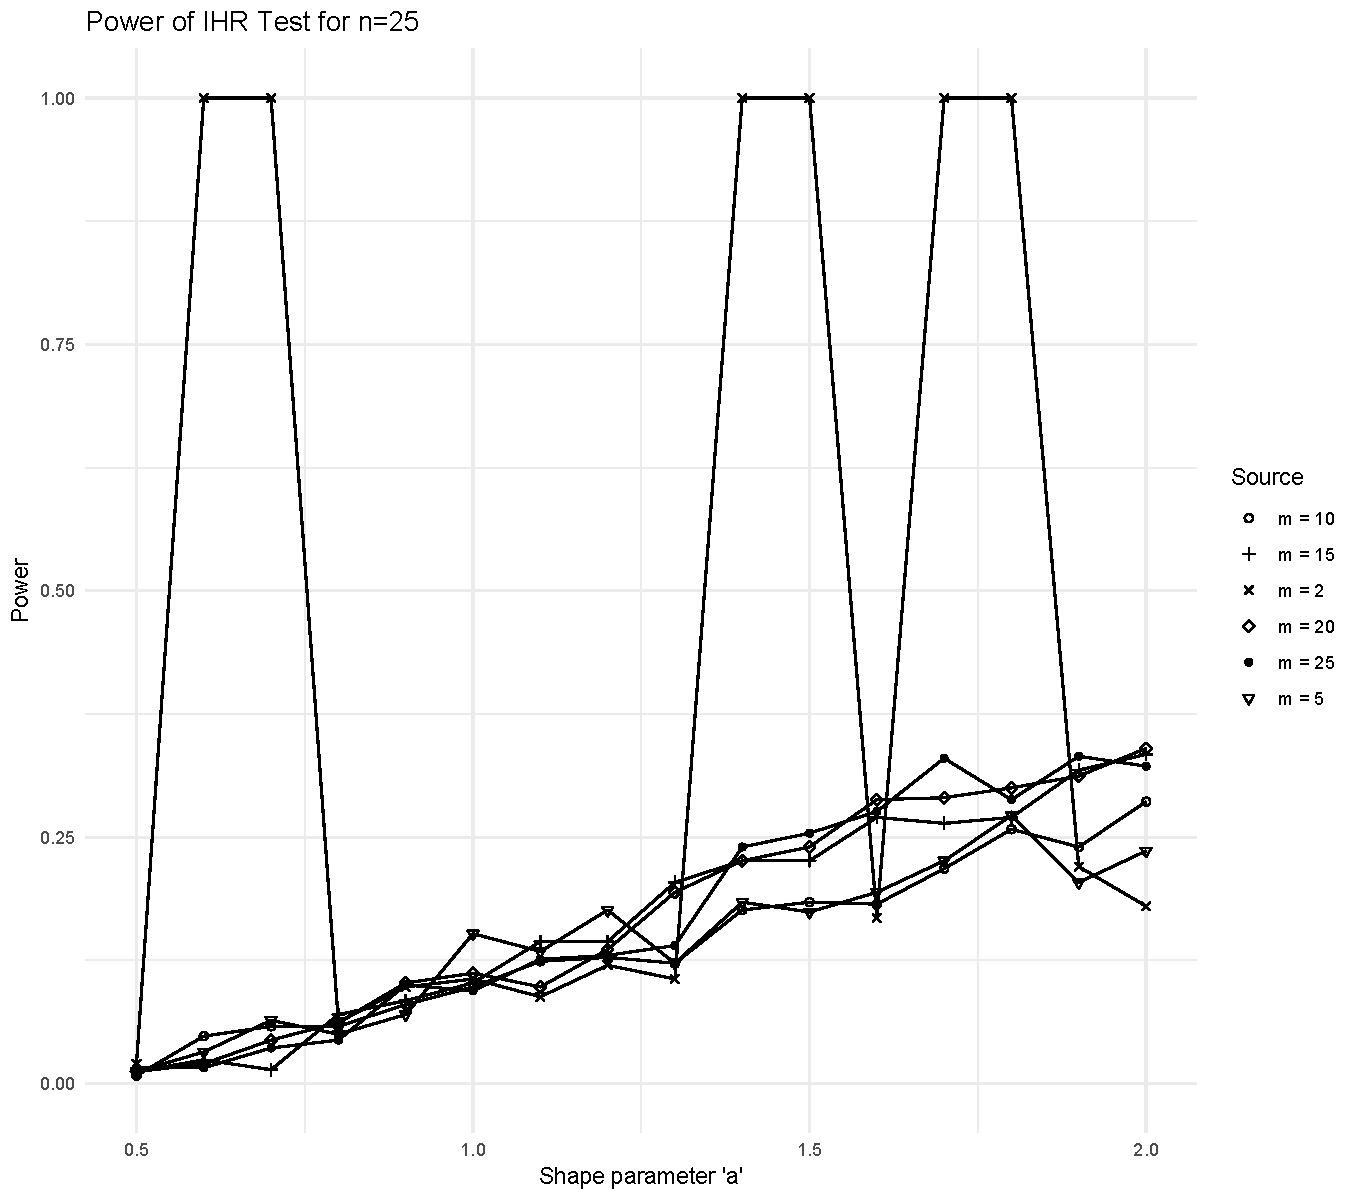
\includegraphics[width=4.5 cm,height=4 cm]{IHR_OS_25.pdf}
			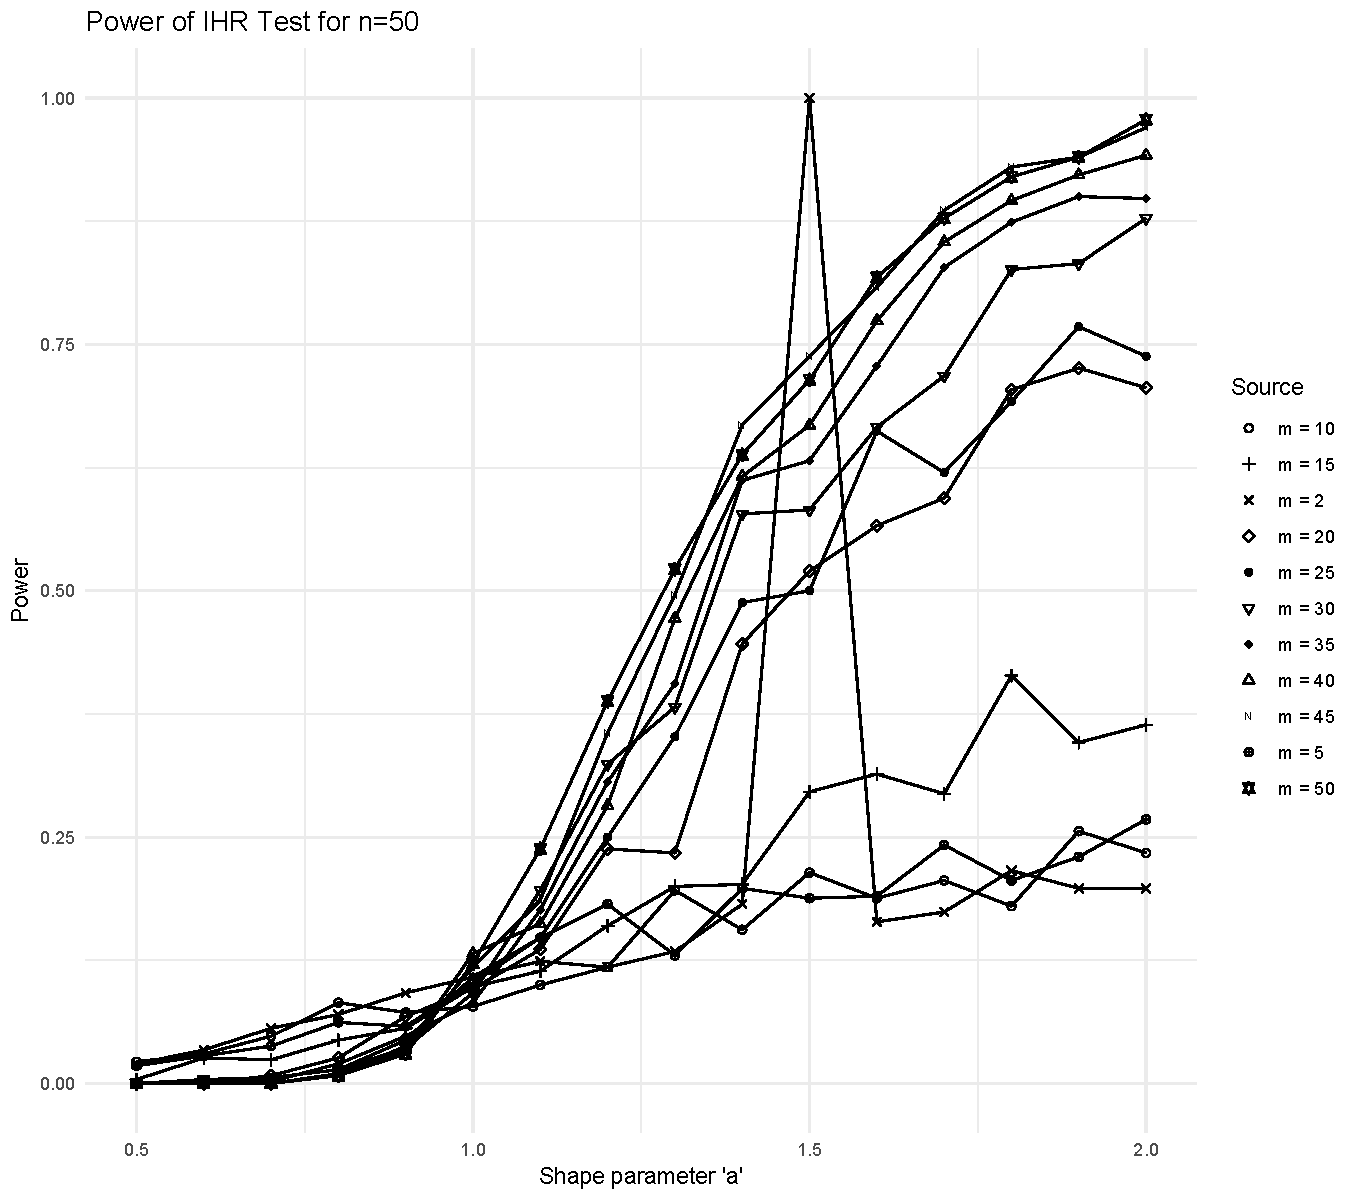
\includegraphics[width=4.5 cm,height=4 cm]{IHR_OS_50.pdf}
			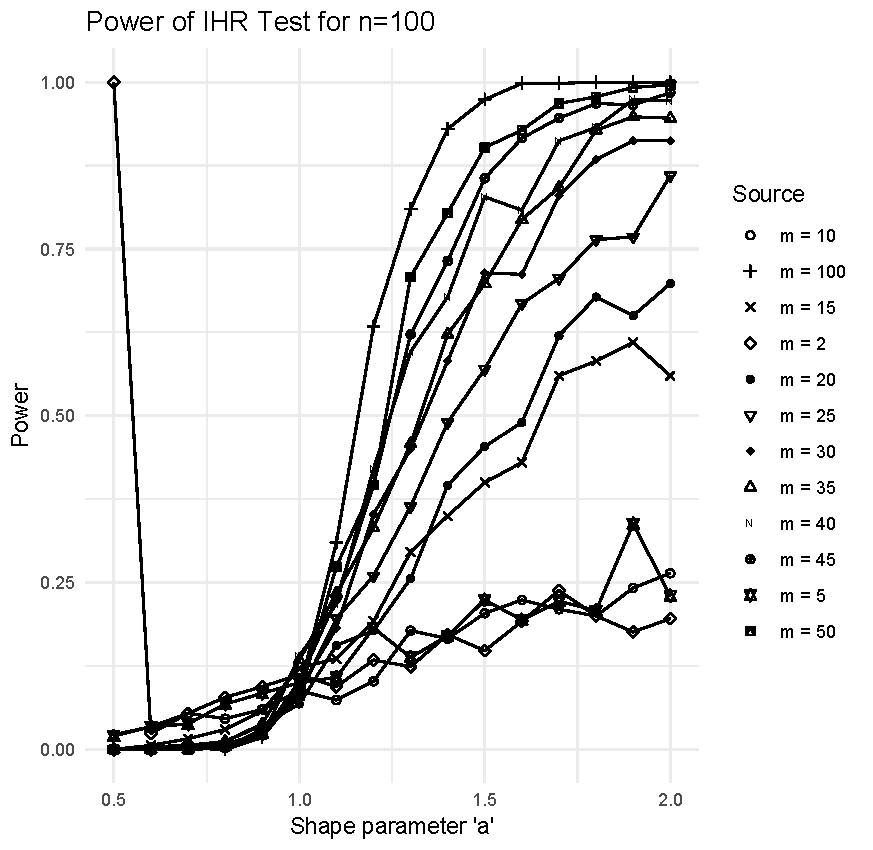
\includegraphics[width=4.5 cm,height=4 cm]{IHR_OS_100.pdf}
			\caption{ $W(0.75,1)$.}
			\label{MSE_Weibull}
		\end{subfigure}
		
		\vspace{0.5em}
		
		% --- Second row: Beta ---
		\begin{subfigure}[b]{\textwidth}
			\centering
			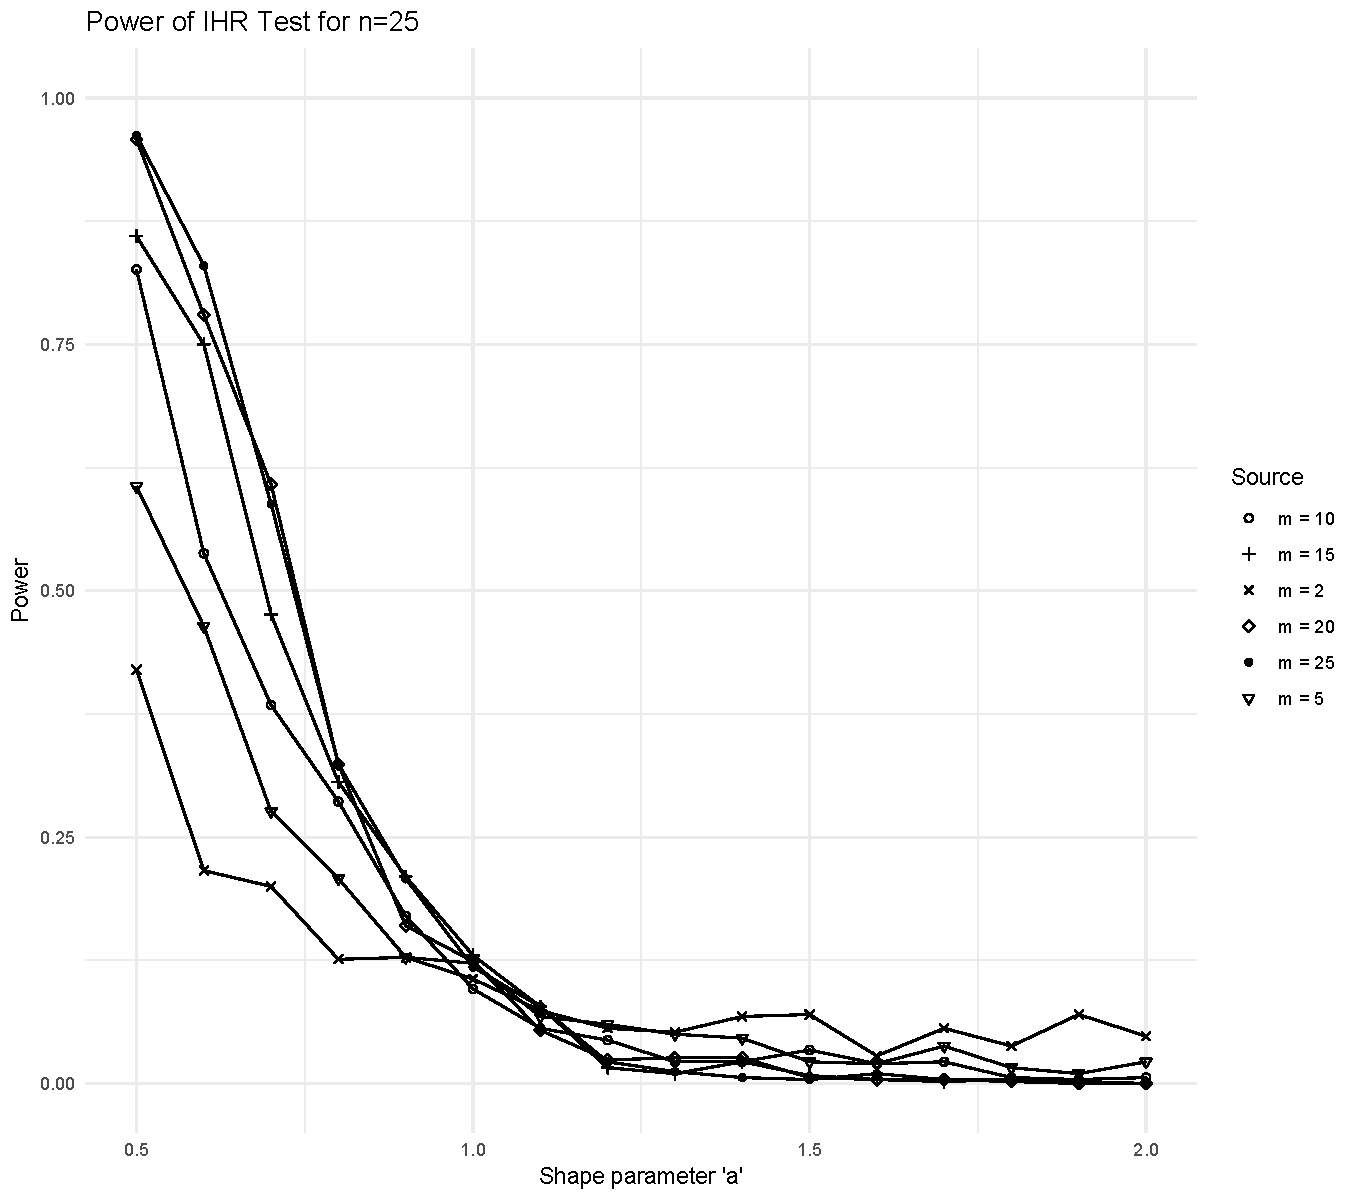
\includegraphics[width=4.5 cm,height=4 cm]{DHR_OS_25.pdf}
			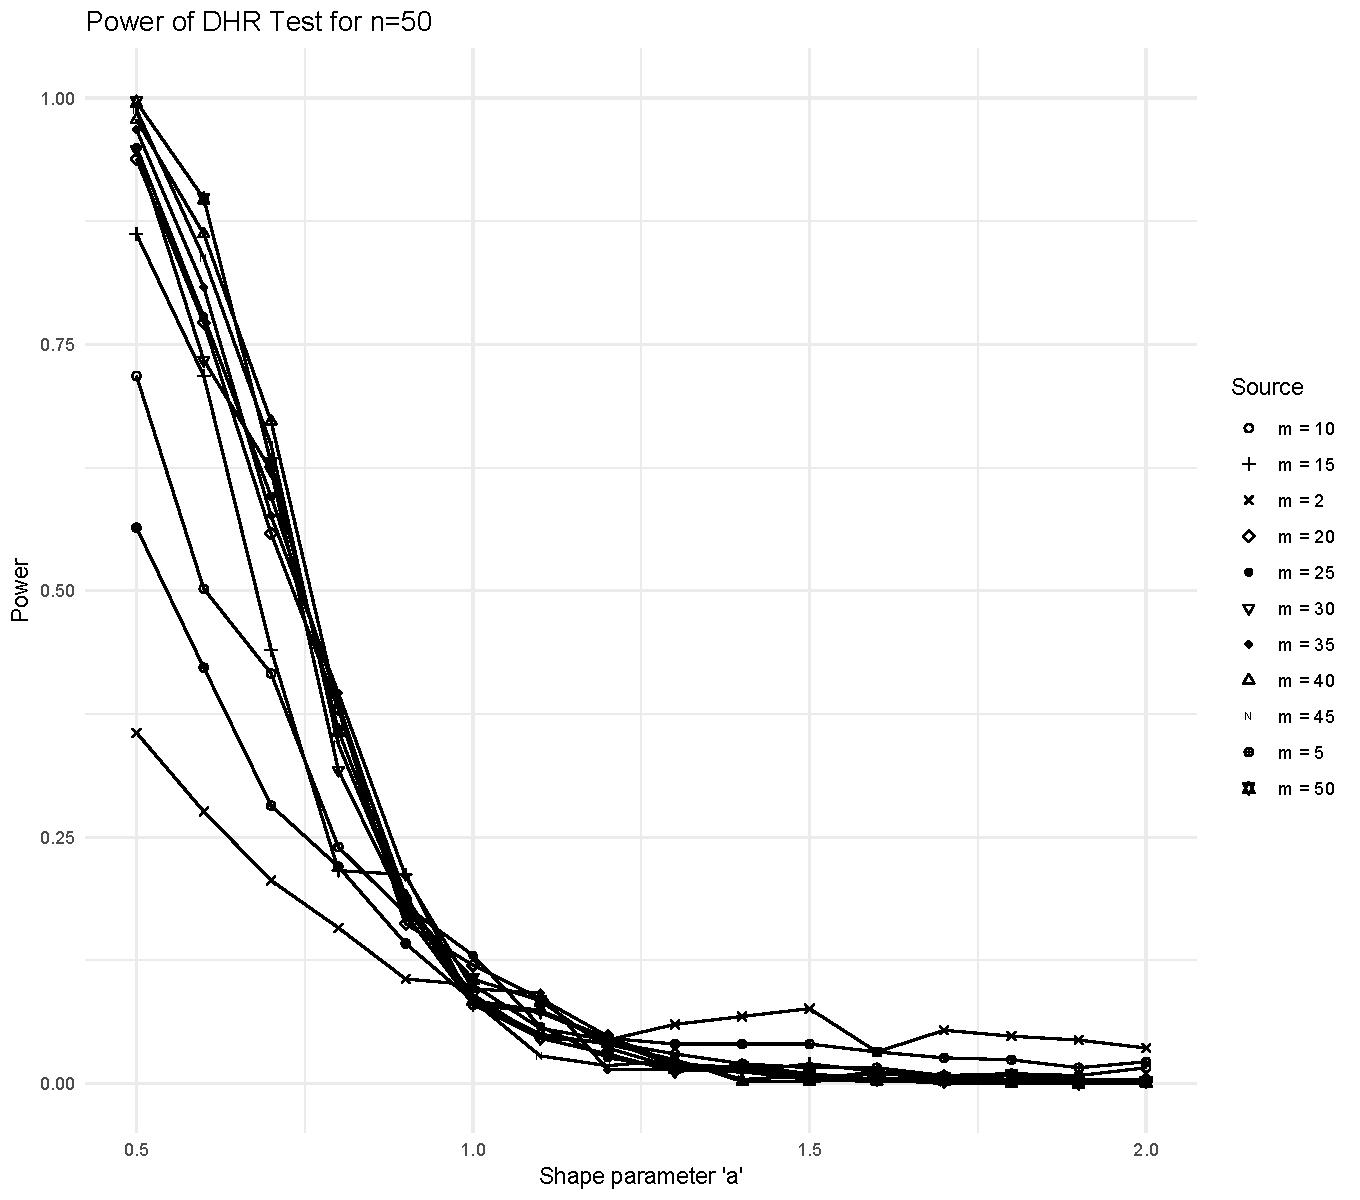
\includegraphics[width=4.5 cm,height=4 cm]{DHR_OS_50.pdf}
			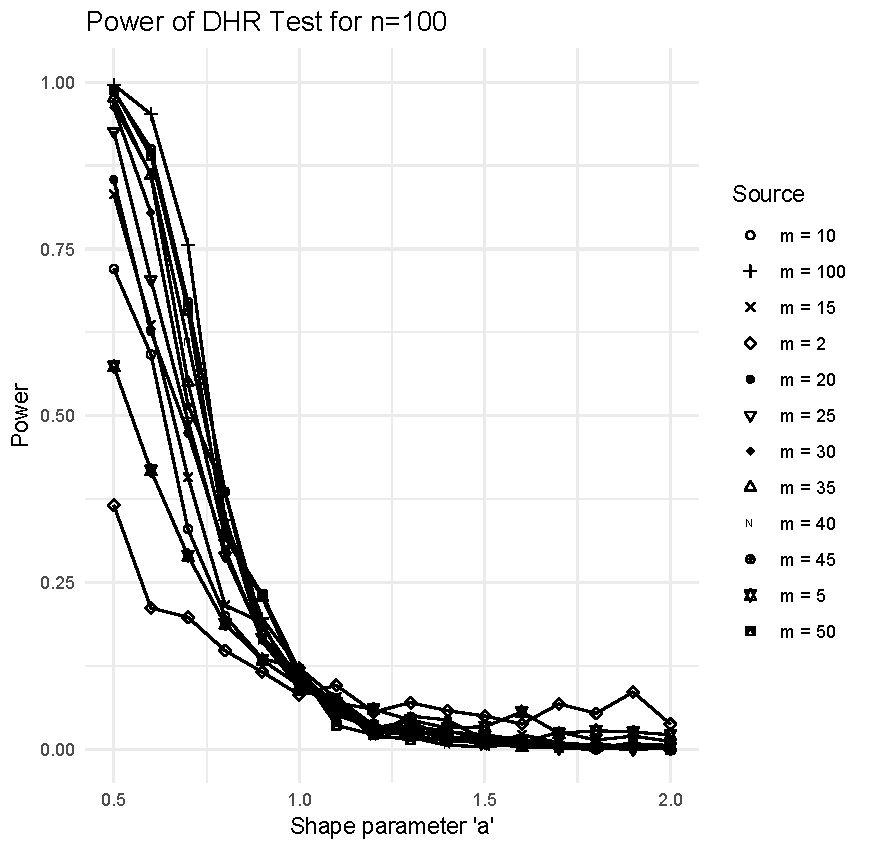
\includegraphics[width=4.5 cm,height=4 cm]{DHR_OS_100.pdf}
			\caption{$B(0.75, 1)$}
			\label{subfig:MSE_beta}
		\end{subfigure}
		
		\caption{Simulation results: Rejection rates of the test based on order statistics for the Weibull distribution \(W(a,1)\), with shape parameter \(a\in[0.5,2]\) and sample sizes \(n\in\{25,50,100\}\).}
		\label{MSE}
	\end{figure}
	
	\begin{figure}[ht]
		\centering
		% --- First row: Weibull ---
		\begin{subfigure}[b]{\textwidth}
			\centering
			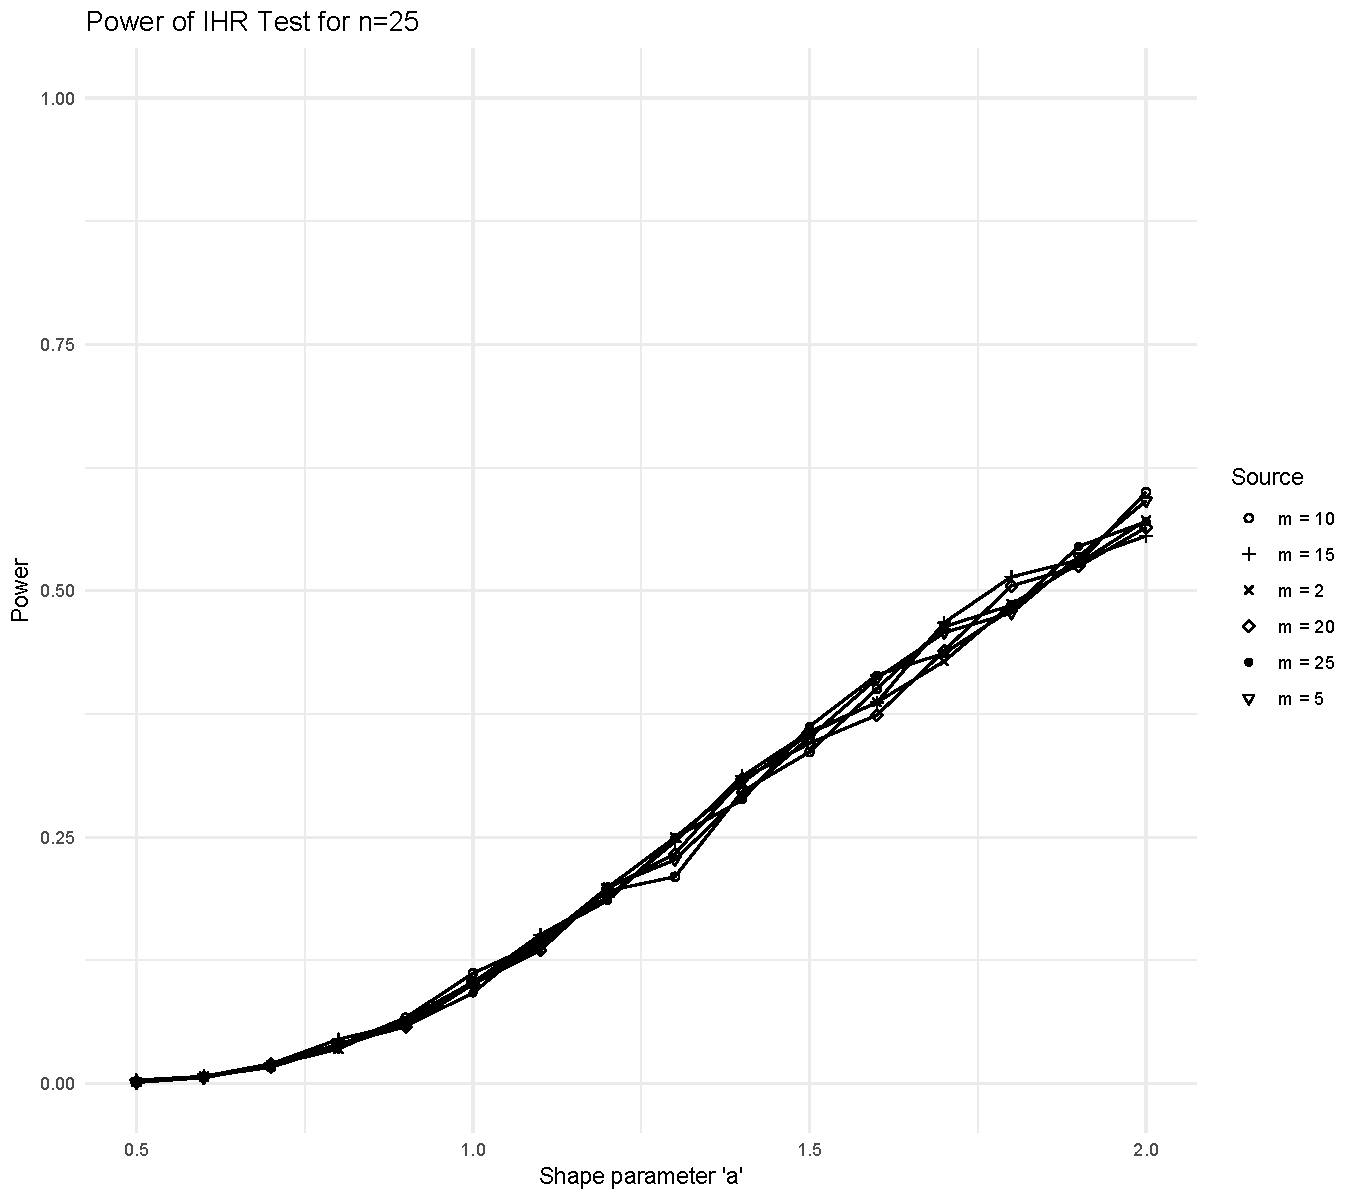
\includegraphics[width=4.5 cm,height=4 cm]{IHR_Records_25.pdf}
			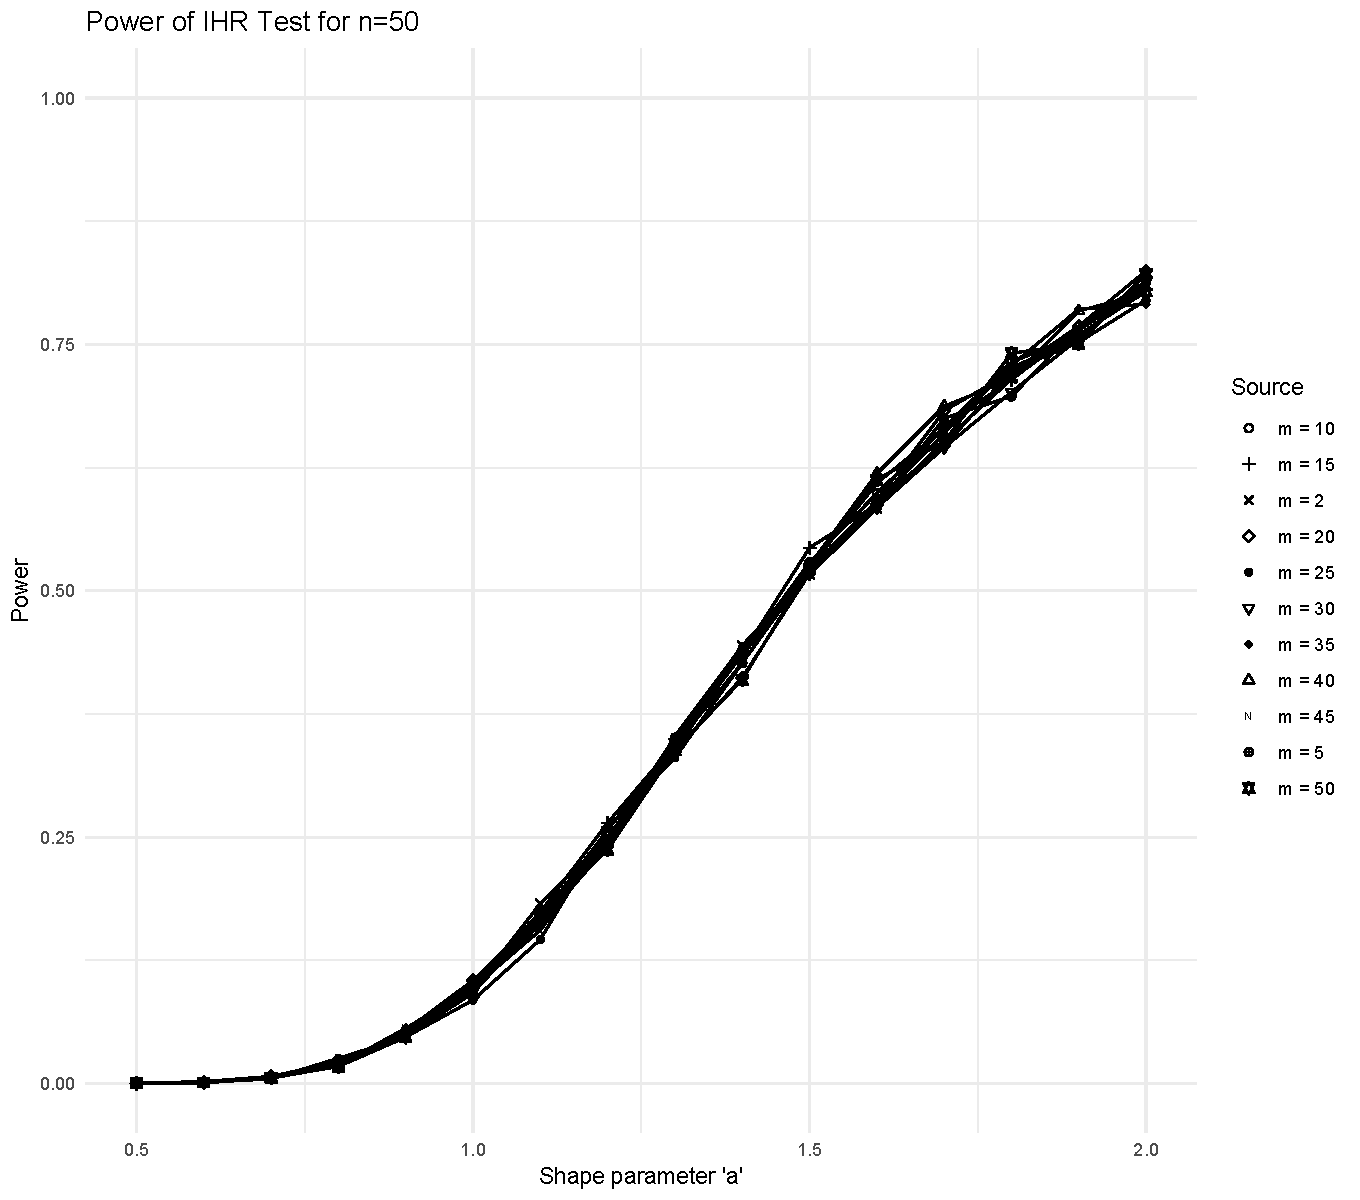
\includegraphics[width=4.5 cm,height=4 cm]{IHR_Records_50.pdf}
			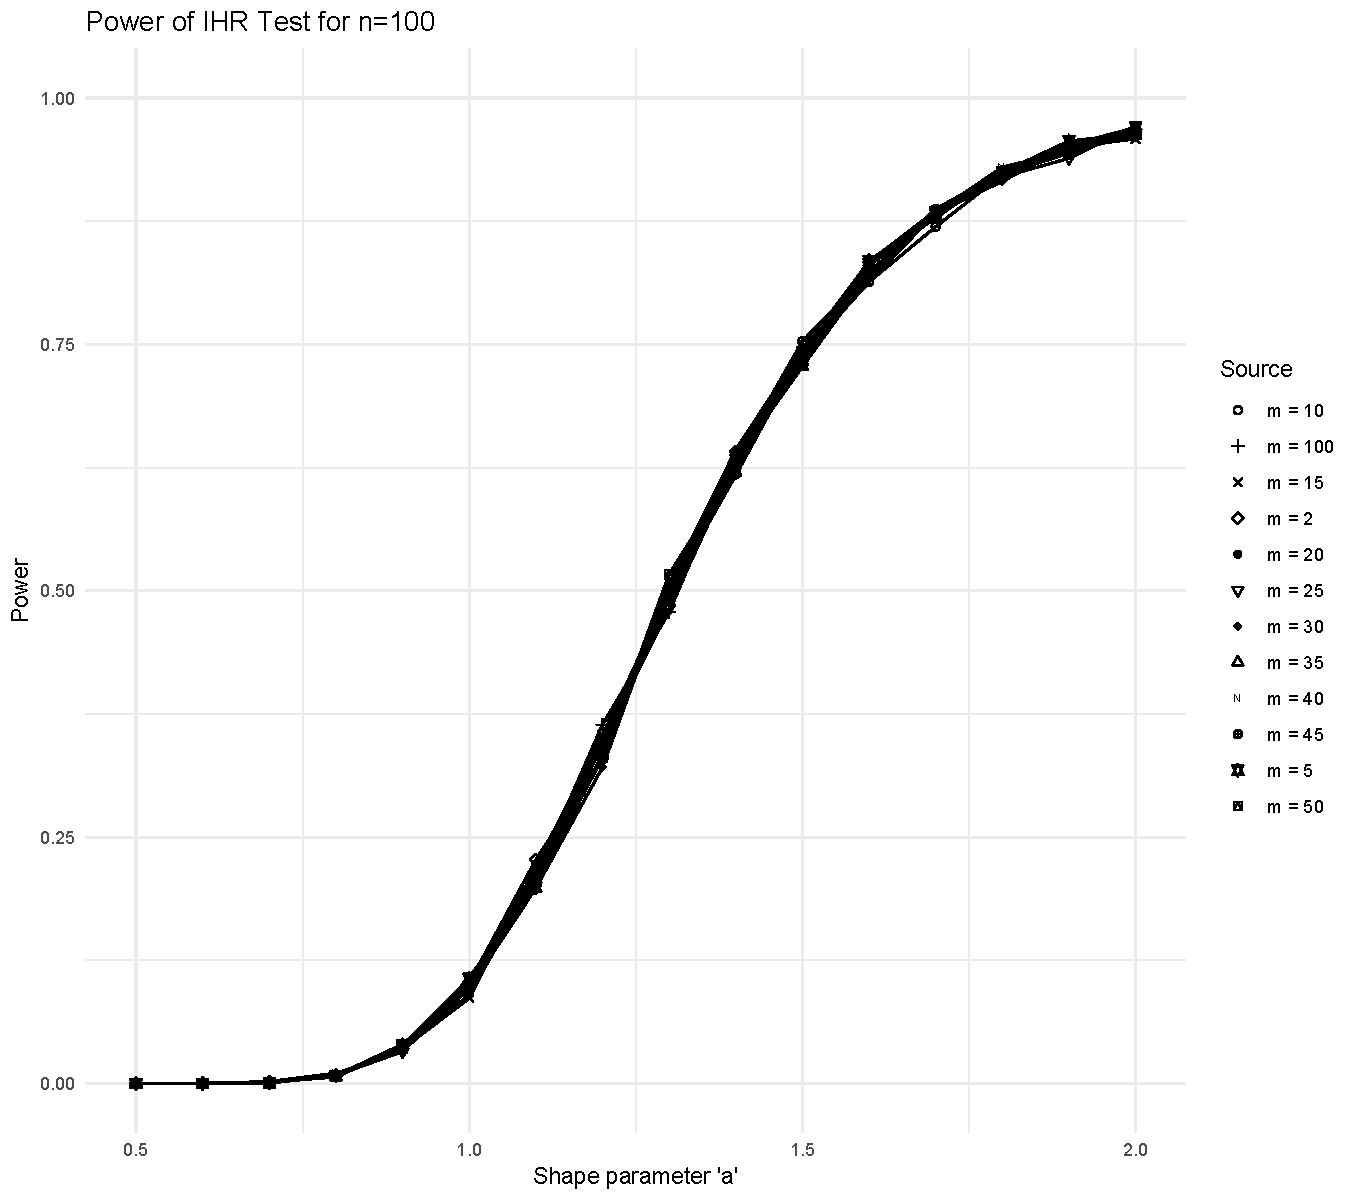
\includegraphics[width=4.5 cm,height=4 cm]{IHR_Records_100.pdf}
			\caption{ IHR.}
			\label{Power_IHR_Records}
		\end{subfigure}
		
		\vspace{0.5em}
		
		% --- Second row: Beta ---
		\begin{subfigure}[b]{\textwidth}
			\centering
			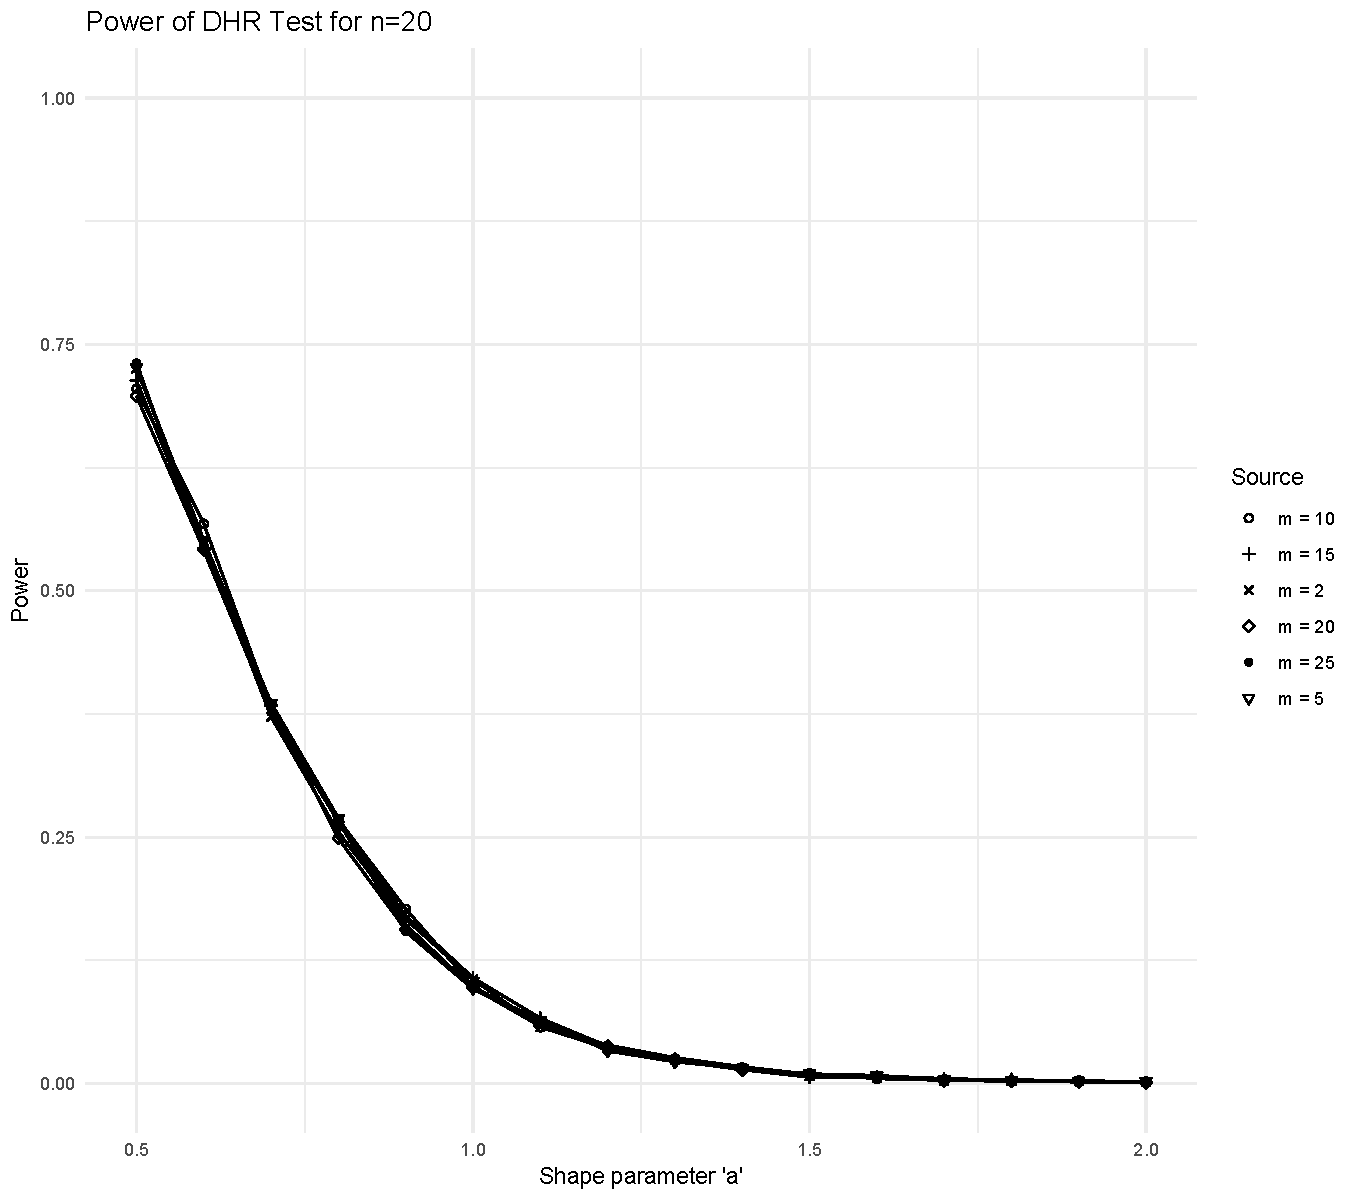
\includegraphics[width=4.5 cm,height=4 cm]{DHR_Records_25.pdf}
			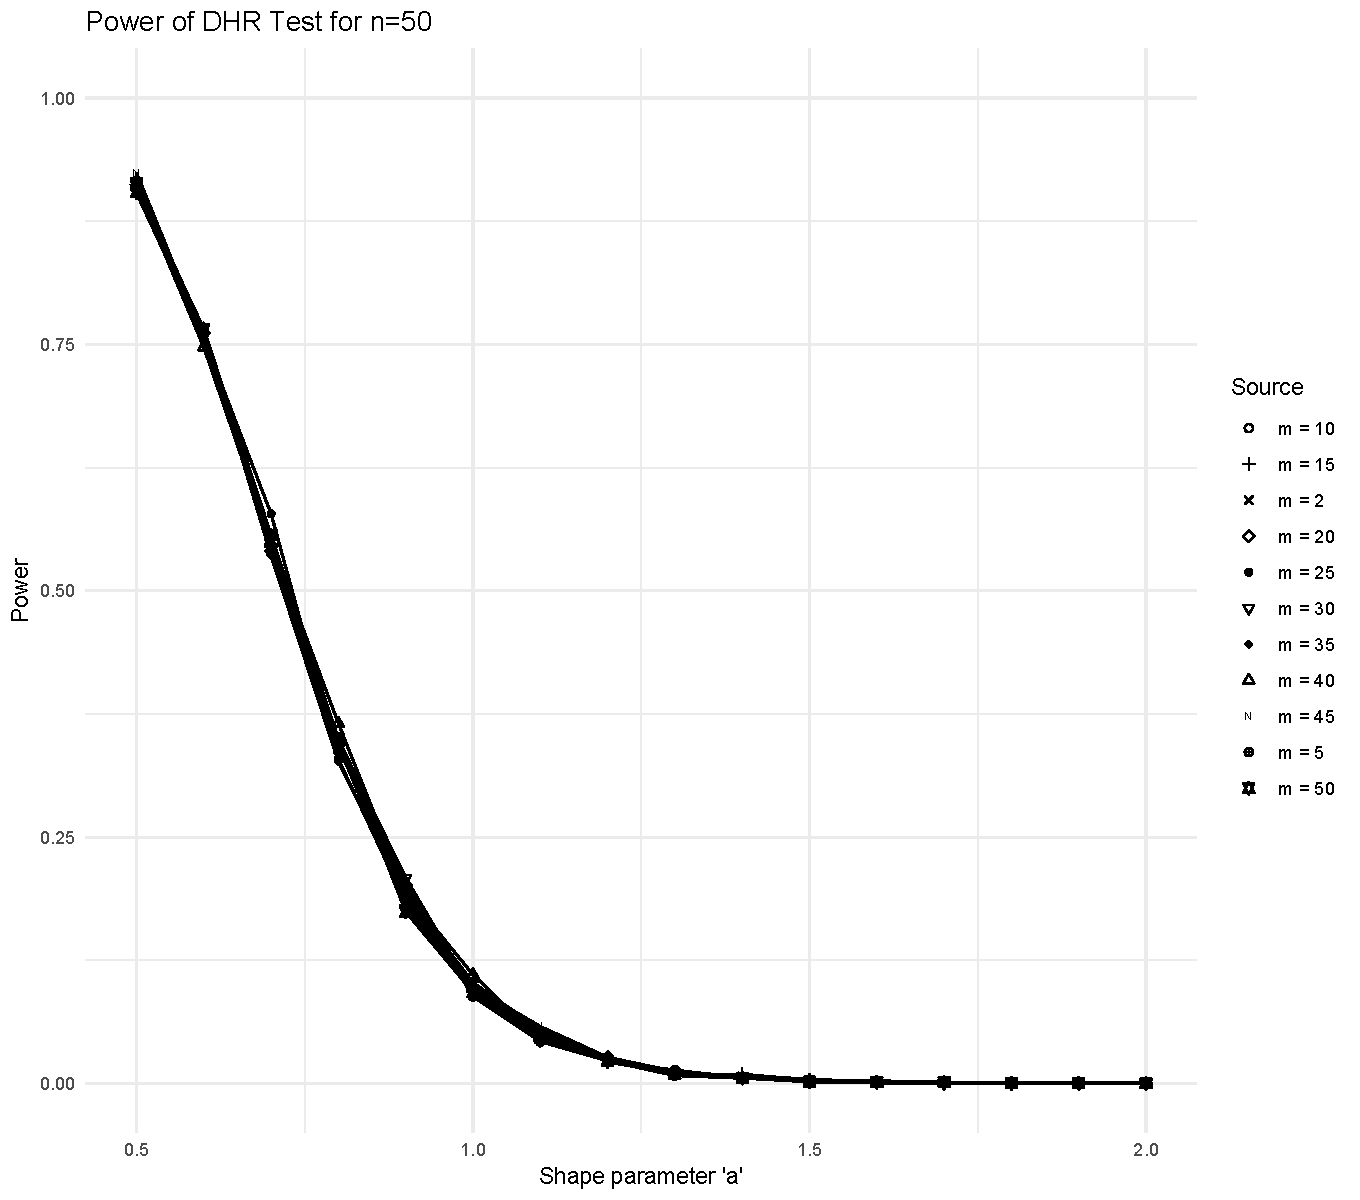
\includegraphics[width=4.5 cm,height=4 cm]{DHR_Records_50.pdf}
			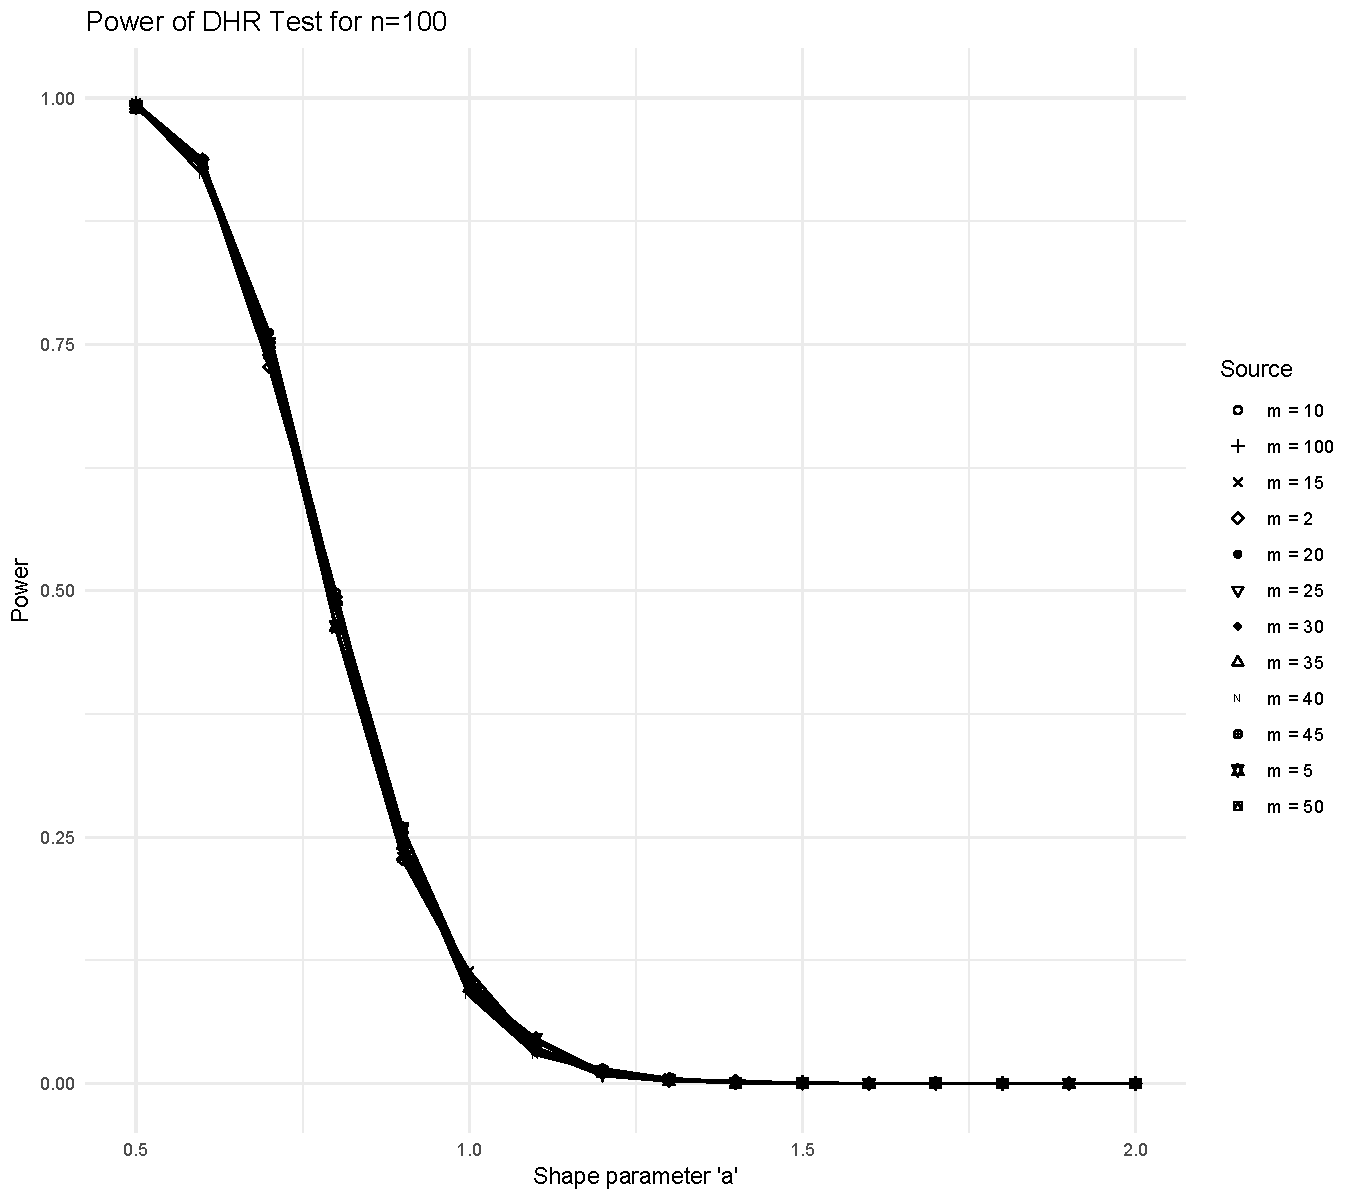
\includegraphics[width=4.5 cm,height=4 cm]{DHR_Records_100.pdf}
			\caption{DHR.}
			\label{Power_DHR_Records}
		\end{subfigure}
		
		\caption{Simulation results: Rejection rates of the test based on upper record values for the Weibull distribution \(W(a,1)\), with shape parameter \(a\in[0.5,2]\) and sample sizes \(n\in\{25,50,100\}\).}
		\label{Power_Records}
	\end{figure}
	\section{Proofs}
	
	\begin{proof}[Proof of Lemma \ref{cdf_U}]
		Let
		\[
		E_j=-\log U_j,\qquad j=1,\ldots,r.
		\]
		Since \(U_j\sim\operatorname{Uniform}(0,1)\), the random variables \(E_1,\ldots,E_r\) are independent and exponentially distributed with rate \(1\). Consequently, \(E_j/\gamma_j\) is exponentially distributed with rate \(\gamma_j\).
		
		Define
		\[
		S_r=\sum_{j=1}^{r}\frac{E_j}{\gamma_j}.
		\]
		By the definition of \(U_{r,\tilde{\gamma}_r}\),
		\[
		U_{r,\tilde{\gamma}_r}=1-e^{-S_r}.
		\]
		Therefore, for \(0<u<1\),
		\[
		\begin{aligned}
			F_{U_{r,\tilde{\gamma}_r}}(u)
			&=\mathbb{P}(1-e^{-S_r}\le u)\\
			&=\mathbb{P}\bigl(S_r\le-\log(1-u)\bigr)\\
			&=1-\mathbb{P}\bigl(S_r>-\log(1-u)\bigr).
		\end{aligned}
		\]
		
		The Laplace transform of \(S_r\) is
		\[
		\mathbb{E}[e^{-sS_r}]
		=\prod_{j=1}^{r}\frac{\gamma_j}{\gamma_j+s},
		\qquad s\ge0.
		\]
		Since the rates \(\gamma_1,\ldots,\gamma_r\) are pairwise distinct, partial-fraction decomposition gives
		\[
		\prod_{j=1}^{r}\frac{\gamma_j}{\gamma_j+s}
		=\sum_{i=1}^{r}
		\frac{\gamma_i}{\gamma_i+s}
		\prod_{\substack{j=1\\j\ne i}}^{r}
		\frac{\gamma_j}{\gamma_j-\gamma_i}.
		\]
		It follows that the survival function of \(S_r\) is
		\[
		\mathbb{P}(S_r>t)
		=\sum_{i=1}^{r}
		\left(
		\prod_{\substack{j=1\\j\ne i}}^{r}
		\frac{\gamma_j}{\gamma_j-\gamma_i}
		\right)e^{-\gamma_i t},
		\qquad t\ge0.
		\]
		Substituting \(t=-\log(1-u)\), we obtain
		\[
		\begin{aligned}
			F_{U_{r,\tilde{\gamma}_r}}(u)
			&=1-\sum_{i=1}^{r}
			\left(
			\prod_{\substack{j=1\\j\ne i}}^{r}
			\frac{\gamma_j}{\gamma_j-\gamma_i}
			\right)e^{\gamma_i\log(1-u)}\\
			&=1-\sum_{i=1}^{r}
			\left(
			\prod_{\substack{j=1\\j\ne i}}^{r}
			\frac{\gamma_j}{\gamma_j-\gamma_i}
			\right)(1-u)^{\gamma_i}.
		\end{aligned}
		\]
		Finally, \(U_{r,\tilde{\gamma}_r}\in(0,1)\) almost surely, so its CDF equals \(0\) for \(u\le0\) and \(1\) for \(u\ge1\). This establishes the result.
	\end{proof}
	
	\begin{proof}[Proof of Lemma \ref{CDF_record}]
		\begin{itemize}
			\item The CDF can be expressed as:
			\[
			\begin{aligned}
				F_{U_{r,\tilde{\gamma}_r}}(u)
				&=P\left(1-\prod_{j=1}^{r}U_j^{1/k}\le u\right)\\
				&=P\left(\prod_{j=1}^{r}U_j\ge(1-u)^k\right)\\
				&=P\left(-\sum_{j=1}^{r}\ln U_j
				\le -k\ln(1-u)\right).
			\end{aligned}
			\]
			
			Since \(U_1,\ldots,U_r\) are i.i.d. \(\operatorname{Uniform}(0,1)\) random variables, the transformed random variables \(-\ln U_1,\ldots,-\ln U_r\) are independent and each follows an exponential distribution with rate \(1\). Consequently, the sum is of $\operatorname{Gamma}(r,1)$ distribution: $-\sum_{j=1}^{r}\ln U_j
			\sim \operatorname{Gamma}(r,1).$ 
			
			
			\item Differentiating the CDF with respect to \(u\) gives the PDF.
			\[
			f_{U_{r,\tilde{\gamma}_r}}(u)=
			\begin{cases}
				\displaystyle
				\frac{k^r}{(r-1)!}
				(1-u)^{k-1}
				\big[-\ln(1-u)\big]^{r-1},
				& 0<u<1,\\[10pt]
				0, & \text{otherwise}.
			\end{cases}
			\]
			Since \(f_{U_{r,\tilde{\gamma}_r}}\) is continuous on \((0,1)\), its boundedness can be determined by examining its behavior at the endpoints. As \(r\geq 1\), the density satisfies
			\[
			\lim_{u\to0^+}f_{U_{r,\tilde{\gamma}_r}}(u)
			=
			\begin{cases}
				k, & r=1,\\
				0, & r>1,
			\end{cases}
			\]
			and is therefore bounded in a neighborhood of \(u=0\). Consequently, it remains to investigate the behavior of the density as \(u\to1^-\) to determine whether it is bounded on \((0,1)\).
			
			
			Next, setting \(t=-\ln(1-u)\), we can rewrite the density as
			\[
			f_{U_{r,\tilde{\gamma}_r}}(u)
			=
			\frac{k^r}{(r-1)!}
			e^{-(k-1)t}t^{r-1},
			\qquad t\to\infty.
			\]
			
			If \(k>1\), the exponential decay dominates the polynomial term, and therefore
			\[
			\lim_{u\to1^-}f_{U_{r,\tilde{\gamma}_r}}(u)=0.
			\]
			Since the density is continuous on \((0,1)\) and has finite limits at both endpoints, it is bounded.
			
			If \(k=1\), the density reduces to
			\[
			f_{U_{r,\tilde{\gamma}_r}}(u)
			=
			\frac{[-\ln(1-u)]^{r-1}}{(r-1)!}.
			\]
			Hence,
			\[
			\lim_{u\to1^-}f_{U_{r,\tilde{\gamma}_r}}(u)
			=
			\begin{cases}
				1, & r=1,\\
				+\infty, & r>1.
			\end{cases}
			\]
		\end{itemize}
	\end{proof}
	\begin{thebibliography}{34}
		\expandafter\ifx\csname natexlab\endcsname\relax\def\natexlab#1{#1}\fi
		\providecommand{\url}[1]{\texttt{#1}}
		\providecommand{\href}[2]{#2}
		\providecommand{\path}[1]{#1}
		\providecommand{\DOIprefix}{doi:}
		\providecommand{\ArXivprefix}{arXiv:}
		\providecommand{\URLprefix}{URL: }
		\providecommand{\Pubmedprefix}{pmid:}
		\providecommand{\doi}[1]{\href{http://dx.doi.org/#1}{\path{#1}}}
		\providecommand{\Pubmed}[1]{\href{pmid:#1}{\path{#1}}}
		\providecommand{\bibinfo}[2]{#2}
		\ifx\xfnm\relax \def\xfnm[#1]{\unskip,\space#1}\fi
		%Type = Article
		\bibitem[{Anis(2013)}]{anis}
		\bibinfo{author}{Anis, M.}, \bibinfo{year}{2013}.
		\newblock \bibinfo{title}{A family of tests for exponentiality against IFR
			alternatives}.
		\newblock \bibinfo{journal}{Journal of Statistical Planning and Inference}
		\bibinfo{volume}{143}, \bibinfo{pages}{1409--1415}.
		%Type = Article
		\bibitem[{Arab et~al.(2025)Arab, Lando and Oliveira}]{landoJAP}
		\bibinfo{author}{Arab, I.}, \bibinfo{author}{Lando, T.},
		\bibinfo{author}{Oliveira, P.}, \bibinfo{year}{2025}.
		\newblock \bibinfo{title}{Inequalities and bounds for expected order statistics
			from convex ordered families}.
		\newblock \bibinfo{journal}{Journal of Applied Probability (to appear)} .
		%Type = Article
		\bibitem[{Barlow et~al.(1963)Barlow, Marshall and Proschan}]{barlow1963}
		\bibinfo{author}{Barlow, R.E.}, \bibinfo{author}{Marshall, A.W.},
		\bibinfo{author}{Proschan, F.}, \bibinfo{year}{1963}.
		\newblock \bibinfo{title}{Properties of probability distributions with monotone
			hazard rate}.
		\newblock \bibinfo{journal}{The Annals of Mathematical Statistics} ,
		\bibinfo{pages}{375--389}.
		%Type = Techreport
		\bibitem[{Barlow and Van~Zwet(1969)}]{barlowzwet}
		\bibinfo{author}{Barlow, R.E.}, \bibinfo{author}{Van~Zwet, W.R.},
		\bibinfo{year}{1969}.
		\newblock \bibinfo{title}{Asymptotic properties of isotonic estimators for the
			generalized failure rate function. {P}art 1: strong consistency}.
		\newblock \bibinfo{type}{Technical Report}. California Univ Berkeley
		{O}perations {R}esearch center.
		%Type = Article
		\bibitem[{Beare(2021)}]{beare2021}
		\bibinfo{author}{Beare, B.K.}, \bibinfo{year}{2021}.
		\newblock \bibinfo{title}{Least favourability of the uniform distribution for
			tests of the concavity of a distribution function}.
		\newblock \bibinfo{journal}{Stat} \bibinfo{volume}{10}, \bibinfo{pages}{e376}.
		%Type = Article
		\bibitem[{Bickel and Doksum(1969)}]{bickel}
		\bibinfo{author}{Bickel, P.J.}, \bibinfo{author}{Doksum, K.A.},
		\bibinfo{year}{1969}.
		\newblock \bibinfo{title}{Tests for monotone failure rate based on normalized
			spacings}.
		\newblock \bibinfo{journal}{The Annals of Mathematical Statistics} ,
		\bibinfo{pages}{1216--1235}.
		%Type = Book
		\bibitem[{Billingsley(2013)}]{billingsley}
		\bibinfo{author}{Billingsley, P.}, \bibinfo{year}{2013}.
		\newblock \bibinfo{title}{Convergence of probability measures}.
		\newblock \bibinfo{publisher}{John Wiley \& Sons}.
		%Type = Article
		\bibitem[{Block et~al.(1998)Block, Savits and Singh}]{block}
		\bibinfo{author}{Block, H.W.}, \bibinfo{author}{Savits, T.H.},
		\bibinfo{author}{Singh, H.}, \bibinfo{year}{1998}.
		\newblock \bibinfo{title}{The reversed hazard rate function}.
		\newblock \bibinfo{journal}{Probability in the Engineering and informational
			Sciences} \bibinfo{volume}{12}, \bibinfo{pages}{69--90}.
		%Type = Article
		\bibitem[{Bryson(1974)}]{bryson}
		\bibinfo{author}{Bryson, M.C.}, \bibinfo{year}{1974}.
		\newblock \bibinfo{title}{Heavy-tailed distributions: properties and tests}.
		\newblock \bibinfo{journal}{Technometrics} \bibinfo{volume}{16},
		\bibinfo{pages}{61--68}.
		%Type = Article
		\bibitem[{Carolan(2002)}]{carolan}
		\bibinfo{author}{Carolan, C.A.}, \bibinfo{year}{2002}.
		\newblock \bibinfo{title}{The least concave majorant of the empirical
			distribution function}.
		\newblock \bibinfo{journal}{Canadian Journal of Statistics}
		\bibinfo{volume}{30}, \bibinfo{pages}{317--328}.
		%Type = Article
		\bibitem[{Chen et~al.(2024)Chen, Embrechts and Wang}]{chen2024}
		\bibinfo{author}{Chen, Y.}, \bibinfo{author}{Embrechts, P.},
		\bibinfo{author}{Wang, R.}, \bibinfo{year}{2024}.
		\newblock \bibinfo{title}{An unexpected stochastic dominance: Pareto
			distributions, dependence, and diversification}.
		\newblock \bibinfo{journal}{Operations Research} .
		%Type = Article
		\bibitem[{Chen and Shneer(2024)}]{chen2024stochastic}
		\bibinfo{author}{Chen, Y.}, \bibinfo{author}{Shneer, S.}, \bibinfo{year}{2024}.
		\newblock \bibinfo{title}{Stochastic dominance for super heavy-tailed random
			variables}.
		\newblock \bibinfo{journal}{arXiv preprint arXiv:2408.15033} .
		%Type = Article
		\bibitem[{Gijbels and Heckman(2004)}]{gibels}
		\bibinfo{author}{Gijbels, I.}, \bibinfo{author}{Heckman, N.},
		\bibinfo{year}{2004}.
		\newblock \bibinfo{title}{Nonparametric testing for a monotone hazard function
			via normalized spacings}.
		\newblock \bibinfo{journal}{Journal of Nonparametric Statistics}
		\bibinfo{volume}{16}, \bibinfo{pages}{463--477}.
		%Type = Article
		\bibitem[{Grenander(1956)}]{grenander}
		\bibinfo{author}{Grenander, U.}, \bibinfo{year}{1956}.
		\newblock \bibinfo{title}{On the theory of mortality measurement: part {II}}.
		\newblock \bibinfo{journal}{Scandinavian Actuarial Journal}
		\bibinfo{volume}{1956}, \bibinfo{pages}{125--153}.
		%Type = Article
		\bibitem[{Groeneboom and Jongbloed(2012)}]{groeneboom2012}
		\bibinfo{author}{Groeneboom, P.}, \bibinfo{author}{Jongbloed, G.},
		\bibinfo{year}{2012}.
		\newblock \bibinfo{title}{Isotonic ${L}_2$-projection test for local
			monotonicity of a hazard}.
		\newblock \bibinfo{journal}{Journal of Statistical Planning and Inference}
		\bibinfo{volume}{142}, \bibinfo{pages}{1644--1658}.
		%Type = Book
		\bibitem[{Groeneboom and Jongbloed(2014)}]{groeneboom2014}
		\bibinfo{author}{Groeneboom, P.}, \bibinfo{author}{Jongbloed, G.},
		\bibinfo{year}{2014}.
		\newblock \bibinfo{title}{Nonparametric estimation under shape constraints}.
		\newblock \bibinfo{number}{38}, \bibinfo{publisher}{Cambridge University
			Press}.
		%Type = Book
		\bibitem[{de~Haan and Ferreira(2006)}]{haan}
		\bibinfo{author}{de~Haan, L.}, \bibinfo{author}{Ferreira, A.},
		\bibinfo{year}{2006}.
		\newblock \bibinfo{title}{Extreme value theory: an introduction}.
		volume~\bibinfo{volume}{3}.
		\newblock \bibinfo{publisher}{Springer}.
		%Type = Article
		\bibitem[{Hall and Van~Keilegom(2005)}]{hall2005}
		\bibinfo{author}{Hall, P.}, \bibinfo{author}{Van~Keilegom, I.},
		\bibinfo{year}{2005}.
		\newblock \bibinfo{title}{Testing for monotone increasing hazard rate}.
		\newblock \bibinfo{journal}{Annals of Statistics} \bibinfo{volume}{33},
		\bibinfo{pages}{1109--1137}.
		%Type = Article
		\bibitem[{Lando(2023)}]{lando2023}
		\bibinfo{author}{Lando, T.}, \bibinfo{year}{2023}.
		\newblock \bibinfo{title}{Testing departures from the increasing hazard rate
			property}.
		\newblock \bibinfo{journal}{Statistics \& Probability Letters}
		\bibinfo{volume}{193}, \bibinfo{pages}{109736}.
		%Type = Article
		\bibitem[{Lando et~al.(2024)Lando, Arab and Eduardo~Oliveira}]{lando2024}
		\bibinfo{author}{Lando, T.}, \bibinfo{author}{Arab, I.},
		\bibinfo{author}{Eduardo~Oliveira, P.}, \bibinfo{year}{2024}.
		\newblock \bibinfo{title}{Nonparametric inference about increasing odds rate
			distributions}.
		\newblock \bibinfo{journal}{Journal of Nonparametric Statistics}
		\bibinfo{volume}{36}, \bibinfo{pages}{435--454}.
		%Type = Article
		\bibitem[{Lando et~al.(2022)Lando, Arab and Oliveira}]{odds}
		\bibinfo{author}{Lando, T.}, \bibinfo{author}{Arab, I.},
		\bibinfo{author}{Oliveira, P.E.}, \bibinfo{year}{2022}.
		\newblock \bibinfo{title}{Properties of increasing odds rate distributions with
			a statistical application}.
		\newblock \bibinfo{journal}{Journal of Statistical Planning and Inference}
		\bibinfo{volume}{221}, \bibinfo{pages}{313--325}.
		%Type = Article
		\bibitem[{Lando et~al.(2023)Lando, Arab and Oliveira}]{landotransform}
		\bibinfo{author}{Lando, T.}, \bibinfo{author}{Arab, I.},
		\bibinfo{author}{Oliveira, P.E.}, \bibinfo{year}{2023}.
		\newblock \bibinfo{title}{Transform orders and stochastic monotonicity of
			statistical functionals}.
		\newblock \bibinfo{journal}{Scandinavian Journal of Statistics}
		\bibinfo{volume}{50}, \bibinfo{pages}{1183--1200}.
		%Type = Book
		\bibitem[{Marshall and Olkin(2007)}]{LifeDist}
		\bibinfo{author}{Marshall, A.W.}, \bibinfo{author}{Olkin, I.},
		\bibinfo{year}{2007}.
		\newblock \bibinfo{title}{Life Distributions}.
		\newblock \bibinfo{publisher}{Springer, New York}.
		%Type = Article
		\bibitem[{Mitra and Anis(2008)}]{mitra2008}
		\bibinfo{author}{Mitra, M.}, \bibinfo{author}{Anis, M.}, \bibinfo{year}{2008}.
		\newblock \bibinfo{title}{An {L}-statistic approach to a test of exponentiality
			against {IFR} alternatives}.
		\newblock \bibinfo{journal}{Journal of Statistical Planning and Inference}
		\bibinfo{volume}{138}, \bibinfo{pages}{3144--3148}.
		%Type = Article
		\bibitem[{M{\"u}ller(2024)}]{muller2024}
		\bibinfo{author}{M{\"u}ller, A.}, \bibinfo{year}{2024}.
		\newblock \bibinfo{title}{Some remarks on the effect of risk sharing and
			diversification for infinite mean risks}.
		\newblock \bibinfo{journal}{arXiv:2411.10139} .
		%Type = Inproceedings
		\bibitem[{Proschan and Pyke(1967)}]{proschan1967}
		\bibinfo{author}{Proschan, F.}, \bibinfo{author}{Pyke, R.},
		\bibinfo{year}{1967}.
		\newblock \bibinfo{title}{Tests for monotone failure rate}, in:
		\bibinfo{booktitle}{Fifth Berkley Symposium}, pp. \bibinfo{pages}{293--313}.
		%Type = Book
		\bibitem[{Resnick(2008)}]{resnick}
		\bibinfo{author}{Resnick, S.I.}, \bibinfo{year}{2008}.
		\newblock \bibinfo{title}{Extreme values, regular variation, and point
			processes}. volume~\bibinfo{volume}{4}.
		\newblock \bibinfo{publisher}{Springer Science \& Business Media}.
		%Type = Book
		\bibitem[{Robertson et~al.(1988)Robertson, Wright and Dykstra}]{robertson1988}
		\bibinfo{author}{Robertson, T.}, \bibinfo{author}{Wright, F.T.},
		\bibinfo{author}{Dykstra, R.L.}, \bibinfo{year}{1988}.
		\newblock \bibinfo{title}{Order restricted statistical inference}.
		\newblock \bibinfo{publisher}{Wiley}.
		%Type = Book
		\bibitem[{Serfling(2009)}]{serfling}
		\bibinfo{author}{Serfling, R.J.}, \bibinfo{year}{2009}.
		\newblock \bibinfo{title}{Approximation theorems of mathematical statistics}.
		\newblock \bibinfo{publisher}{John Wiley \& Sons}.
		%Type = Book
		\bibitem[{Shaked and Shantikumar(2007)}]{shaked}
		\bibinfo{author}{Shaked, M.}, \bibinfo{author}{Shantikumar, J.G.},
		\bibinfo{year}{2007}.
		\newblock \bibinfo{title}{Stochastic Orders}.
		\newblock \bibinfo{publisher}{Springer, New York}.
		%Type = Article
		\bibitem[{Van~Zwet(1964)}]{vanzwet1964}
		\bibinfo{author}{Van~Zwet, W.R.}, \bibinfo{year}{1964}.
		\newblock \bibinfo{title}{Convex transformations of random variables}.
		\newblock \bibinfo{journal}{MC Tracts} .
		%Type = Article
		\bibitem[{Van~Zwet(1980)}]{zwet1980}
		\bibinfo{author}{Van~Zwet, W.R.}, \bibinfo{year}{1980}.
		\newblock \bibinfo{title}{A strong law for linear functions of order
			statistics}.
		\newblock \bibinfo{journal}{The Annals of Probability} \bibinfo{volume}{5},
		\bibinfo{pages}{986--990}.
		%Type = Article
		\bibitem[{Wellner(1977)}]{wellner}
		\bibinfo{author}{Wellner, J.A.}, \bibinfo{year}{1977}.
		\newblock \bibinfo{title}{A {G}livenko-{C}antelli theorem and strong laws of
			large numbers for functions of order statistics}.
		\newblock \bibinfo{journal}{The Annals of Statistics} \bibinfo{volume}{5},
		\bibinfo{pages}{473--480}.
		%Type = Article
		\bibitem[{Zimmer et~al.(1998)Zimmer, Wang and Pathak}]{zimmer}
		\bibinfo{author}{Zimmer, W.J.}, \bibinfo{author}{Wang, Y.},
		\bibinfo{author}{Pathak, P.K.}, \bibinfo{year}{1998}.
		\newblock \bibinfo{title}{Log-odds rate and monotone log-odds rate
			distributions}.
		\newblock \bibinfo{journal}{Journal of quality technology}
		\bibinfo{volume}{30}, \bibinfo{pages}{376--385}.
		
	\end{thebibliography}
	
\end{document}